\chapter{Collision SPH}
\label{chap:csph}



\section{Introduction}
\label{sec:intro}
In the current chapter we model the collision between elastic bodies. Modeling
the collision among elastic solids allows us to handle the interaction between
the target and the impactor when they are assumed as elastic or elastic-plastic.
An SPH based solution leads to unphysical interactions in modeling the collision
of objects when they are close by but not touching. Further, SPH model does not
incorporate friction between the colliding bodies. In the current chapter, a
contact force model is incorporated into the existing solver to handle the
interaction between the colliding solids. Specifically, we consider bodies with
arbitrary shapes.


The collision of arbitrary solid bodies occurs everywhere around us. Apart
from the elastic collision of bodies, other important examples include surface
erosion, waterjet machining \citep{natarajan2020abrasive}, and machining
processes \citep{islam2020numerical} to note a few. It is important to be able
to simulate such problems accurately.

% When body A discretized into n particles is colliding a body B which is
% discretized in to m particles, above techniques use the particles in B to
% compute the accelerations of density and velocity of particles in A. A few
% drawbacks of this approach is, the bodies come in to contact even when the
% bodies are physically not touching, and the no frictional modeling is modeled.
% \cite{yan2021simulation} has proposed a interfacial SPH scheme , where each
% elastic body uses their own particles in computation of divergence, momentum
% and strain rate. While, the bodies interact by a repulsive force inspired from
% Ansys. Where they have shown the improvement on modeling the collision with
% different examples. Yan has considered Gray SPH which is not so great with
% kernel invariance as it shows tensile instability with a few kernels as shown
% by Roth 2020. Also the contact force model didn't incorporate the frictional
% part of the collision. Further the contact force has a influence of 2h radius,
% implies there would be a force acting on the interacting bodies though they
% are not touching physically.

% The contact force model used in Yan is inspired from ANSYS model and is given.
% A similar work is done by \cite{vyas2021collisional}, where the author models
% the interaction between a circular rigid body impacting a target surface. In
% his work, author proposes a non-linear penalty based force model which could
% handle friction as well and studies the rebounding characteristic of the
% impactor. Here, the author studies the post collision behaviour of the
% circular rigid body which is interacting the elastic plastic solid at
% different incident angles. \cite{mohseni2021particle} proposed an advanced
% version of the collision model where he models the interaction between a rigid
% body with a brittle solids and models the erosion of the brittle solid.

% Finally the current model comes into place only when the material interfaces
% are touching unlike what Yan's contact force model and conventional SPH. We
% also check the invariance of the current scheme in modeling the collisions for
% different types of kernels used.


In the current work, the collision between elastic solids is modeled using a
penalty-based contact force model. A contact force based approach for collision
handling will eliminate the spurious interaction between bodies, which occurs
while modeling with an SPH-based model. Unlike the approach of
\citep{yan2021simulation}, the proposed contact force model can handle friction
between the solids as well. The bodies themselves are elastic and this is
simulated using the CTVF SPH method \citep{adepu2021corrected}. The
penalty-based force considered here is the one proposed by
\cite{mohseni2021particle}. In the original model proposed by
\citep{mohseni2021particle}, the contact force is between a primary body and a
secondary body. In \citep{mohseni2021particle}, the primary body is usually
treated as the rigid body and the body on which the erosion is simulated is
treated as secondary. It is not clear what would happen if both bodies were
elastic or if there is no clear way to distinguish between a primary and
secondary body. We explore these questions in the present work. The work of
\cite{mohseni2021particle} takes inspiration from that of
\cite{vyas2021collisional} where too there is a clear distinction between
primary and secondary bodies. \cite{vyas2021collisional} also consider the
collision between a rigid and elastic body. In the present work we only
implement the collision model of \citep{mohseni2021particle} due to its
simplicity. The model proposed by \cite{vyas2021collisional} is more complex to
implement. Several examples are simulated to validate the current scheme,
ranging from simulations compared with FEM, analytical results as well as
experimental. We next look at the numerical method used to model the collision
among the elastic solids.


\FloatBarrier%
\section{SPH model for structural dynamics}
\label{sec:SPH-model-for-structural-dynamics}

\subsection{Discrete governing equations}
\label{sec:discrete-governing-equations}
We follow the CTVF formulation developed in \cref{chap:ctvf} to handle the
structural dynamics of the solid. The governing equations of including the new
contact force term are:
\begin{equation}
\label{eqn:sph-continuity}
  \frac{\tilde{d}\rho_a}{dt} = \sum_{b \in A} \; \frac{m_b}{\rho_{b}} \; (
  \rho_{a} \; \tilde{\ten{u}}_{ab} \; + \;
  (\rho \; (\tilde{\ten{u}} \; - \;
  \ten{u}))_{ab}) \; \cdot \nabla_{a} W_{ab},
\end{equation}
\begin{equation}
\label{eqn:sph-momentum}
  \frac{\tilde{d}\ten{u}_{a}}{dt} = - \sum_{b \in A} m_b \bigg[
  \bigg(\frac{p_a}{\rho_a^2} + \frac{p_b}{\rho_b^2}\bigg) \ten{I} -
  \bigg(\frac{\teng{\sigma}^{'}_{a}}{\rho_a^2} +
  \frac{\teng{\sigma}^{'}_{b}}{\rho_b^2} + \Pi_{ab} \ten{I} \bigg) \bigg]  \cdot \nabla_{a} W_{ab} +
  \ten{g}_{a} + \frac{1}{m_a}\sum_{b \in B} \ten{F}^{\text{cont}}_{a \leftarrow b}.
\end{equation}
Here, $\ten{F}^{cont}_{a}$ is the force acting on particle $a$ due to
\begin{figure}[!htpb]
  \centering
  \includegraphics[width=1.0\textwidth]{images/csph/images/contact_force/contact_force_description}
  \caption{Bodies under collision which are divided into primary and
    secondary.}
\label{fig:bodies_under_collision}
\end{figure}
contact with the other elastic bodies which will be discussed in
\cref{sec:contact-algorithm}. We follow \cref{chap:ctvf} in handling the
boundaries , in updating the state of the bodies to the next stage, while
transporting particles with a PST.


\FloatBarrier%
\section{Contact algorithm}
\label{sec:contact-algorithm}
In the current work we have utilized the contact force model proposed by
\cite{mohseni2021particle}. The force acting on a particle $a$ of body A due
to the interaction with the particles of body $B$ can be resolved into a
normal and tangential component. The normal force component is utilised to
make sure that the particles of different bodies do not penetrate into each
other, while the tangential component is used to model the friction between
the interacting solids. According to \cite{mohseni2021particle}, we divide the
bodies under interaction into primary and secondary bodies, as shown in
\cref{fig:bodies_under_collision}.
% In usual DEM to compute the force on particle i of body A, the force is
% computed by considering the overlap of particle i with each and every
% particle of body j by considering the particle j to be spherical. This leads
% to unphysical modeling of contact force when the body is interacting with a
% flat surface or surfaces which are not spherical by nature. The current
% contact force is surface aware. The force on particle $i$ is computed by
% equation
The normal force ($\teng{F}_a^{n}$) on
particle $a$ due to the interaction with the particles $b$ of body $B$ is
computed as,
\begin{equation}
  \label{eq:contact-algorithm-normal}
  \ten{F}_a^n = k_r \delta_{n^{c}}^{a} \ten{n}_a^{c}.
\end{equation}
Here, the overlap $\delta_{n^{c}}^{a}$ is computed using
\begin{equation}
  \label{eq:csph:cf-overlap}
  \delta_{n^{c}}^{a} = \Delta x - d_a,
\end{equation}
where,
\begin{equation}
  \label{eq:cf-distance-computation}
  d_a = \frac{
    \displaystyle\sum\limits_{b = 1}^{\text{NP}^{b}} \;
    \big( \ten{n}_a^{c} \cdot \ten{r}_{ab} \big)  \frac{m_b}{\rho_b} W_{ab}}
  {
    \displaystyle\sum\limits_{b = 1}^{\text{NP}^{b}} \;
    \frac{m_b}{\rho_b} W_{ab}},
\end{equation}
and the normal contact vector $\ten{n}_a^{c}$ is computed using
\begin{equation}
  \label{eq:cf-normal-vector}
  \ten{\hat{n}}_a^{c} = \frac{
    \displaystyle\sum\limits_{b = 1}^{\text{NP}^{b}} \;
    \frac{\ten{r}_{ab}}{r_{ab}}  \frac{m_b}{\rho_b} W_{ab}}
  {
    \displaystyle\sum\limits_{b = 1}^{\text{NP}^{b}} \;
    \frac{m_b}{\rho_b} W_{ab}},
\end{equation}
\begin{equation}
  \label{eq:cf-normal-vector}
  \ten{n}_a^{c} = \frac{\teng{\hat{n}}_a^{c}}{||\teng{\hat{n}}_a^{c}||}.
\end{equation}
\begin{figure}[!htpb]
  \centering
  \includegraphics[width=0.3\textwidth]{images/csph/images/contact_force/contact_force_delta_computation}
  \caption{Pictorial representation of distance between a particle and a body.}
\label{fig:contact_force_delta_computation}
\end{figure}
Where $\Delta x$ being the initial spacing between the particles, $k_r$ is the
normal spring stiffness coefficient. \Cref{fig:contact_force_delta_computation}
shows $\Delta x$ and $d_a$ quantities, respectively. Note that while computing
the overlap of particle $a$ with the body $B$ we have computed an effective
overlap, rather than per particle interaction. This is effectively able to model
the interaction between non-smooth surfaces in contrast with particle-particle
force computation.

\subsection{Tangential force computation}
\label{sec:tangential-force-computation}
We associate a tangential spring attached to particle $a$
($|\Delta \textit{\textbf{l}}_a|$) and body $B$ to compute the tangential force
($\ten{F}_{a}^{t}$), which initially has a magnitude of zero
($|\Delta \textit{\textbf{l}}_a|=0$). The tangential spring is activated when
the particle comes into contact with body $B$. The tangential force is
history-dependent. The contact friction force is proportional to the tangential
spring displacement, which is integrated over the contact time as
\begin{equation}
  \label{eq:tangential-force}
  \ten{F}_{a}^{t^{n+1}} =
  -k_f \Delta \textit{\textbf{l}}_a^{\,n + 1} =
  -k_f \big[\big(\Delta {\textit{\textbf{l}}}_a^{\,n} \
  + \ten{v}_{ab}^{n + 1} \Delta t\big) \cdot \ten{t}_a^{n + 1} \big] \
  \ten{t}_a^{n + 1},
\end{equation}
where $\Delta t$ is the time step, $\ten{v}_{ab} = \ten{v}_{a} - \ten{v}_b$ is
the relative velocity of the primary particle $a$ with respect to the closest
secondary particle $b$, $\ten{t}_a$ is the tangential unit vector, and $k_f$ is the tangential spring stiffness
coefficient. Here, $n$ and $n+1$ represent the times which are $\Delta t$ apart.
The tangential unit vector is computed by,
\begin{equation}
  \label{eq:tangential-vect}
  \ten{t}_a = \frac{\ten{v}_{ab} - (\ten{v}_{ab} \cdot \ten{n}_a^{c}) \ten{n}_a^{c}}{|\ten{v}_{ab} - (\ten{v}_{ab} \cdot \ten{n}_a^{c}) \ten{n}_a^{c}|}.
\end{equation}

The tangential force is coupled to the normal force through the Coulomb's law,
\begin{equation}
  \label{eq:Coulomb-law}
  \ten{F}_{a}^{t} = \min(\mu |\ten{F}_{a}^{n}|, |\ten{F}_{a}^{t}|) \
  \frac{\ten{F}_{a}^{t}}{|\ten{F}_{a}^{t}|}.
\end{equation}
This allows us to impose the sliding friction condition between the
interacting solids. Finally, the total force acting on the particle $a$ due to
the interaction with body $B$ is:
\begin{equation}
  \label{eq:contact-force}
  \ten{F}_{a}^{\text{cont}} = \ten{F}_{a}^{n} + \ten{F}_{a}^{t}
\end{equation}

\begin{figure}[!htpb]
  \centering
  \includegraphics[width=0.3\textwidth]{images/csph/images/contact_force/contact_force_description_3}
  \caption{Force transfer to the secondary particles $b$ from the primary body particle $a$}
\label{fig:secondary_particle_contact_foce_transfer}
\end{figure}
An equal and opposite force of the same magnitude is applied to the closest
secondary particle $b$ of $a$ as shown in
\cref{fig:secondary_particle_contact_foce_transfer},
\begin{equation}
  \label{eq:contact-force}
  \ten{F}_{b}^{\text{cont}} = - \ten{F}_{a}^{\text{cont}}.
\end{equation}

% The force on the particle $j$ is evaluated, on the
% body belonging to the secondary surface is as follows. Particles belonging to
% the secondary surface ($j$) which are at a distance less than the initial
% spacing ($l_0$) share the force exerted on particle i, as following:
% \begin{equation}
%   \label{eq:cf-overlap}
%   F^{ij} = - F^{i} w^{ij},
% \end{equation}
% where $w^{ij}$ is defined as
% \begin{equation}
%   \label{eq:cf-overlap}
%   w^{ij} = \frac{n^{i} \cdot \hat{\ten{r}}^{ij}}{\sum_j n^{i} \cdot \hat{\ten{r}}^{ij}}
% \end{equation}

The current contact force model is sensitive towards the primary body chosen
to compute the forces, i.e., the force acting on the particles is not the same
when the primary bodies are interchanged. In the current work we have explored
the behaviour of the current contact force model when different bodies are
chosen as primary and secondary. Simulations such as, a rectangular solid
sliding down an inclined plane, and a symmetric collision between elastic
solids are two examples, where we have investigated how the bodies would behave
when different bodies are chosen as primary.
% , as shown in \cref{fig:primary-secondary-demonstration}.
% \begin{figure}[!htpb]
%   \centering
%   \begin{subfigure}{0.48\textwidth}
%     \centering
%     \includegraphics[width=1.0\textwidth]{images/csph/images/primary_vs_secondary/sliding}
%     \subcaption{A sliding body.}%\label{fig:rings:ipst-nu-0.47-0}
%   \end{subfigure}
%   \begin{subfigure}{0.48\textwidth}
%     \centering
%     \includegraphics[width=1.0\textwidth]{images/csph/images/primary_vs_secondary/symmetric_collision}
%     \subcaption{A symmetric collision between rectangular solids.}%\label{fig:rings:ipst-nu-0.47-1}
%   \end{subfigure}
%   \caption{Examples used to explore the importance of choosing a primary.}
% \label{fig:primary-secondary-demonstration}
% \end{figure}

% =========================================== %
% ------ Results start ---------------------- %
% =========================================== %

\FloatBarrier%
\section{Results and discussion}
\label{sec:results}
In the interest of reproducibility and easier ability
for researchers to build on this work, our code is open source and can be
found at \url{https://gitlab.com/pypr/collision_sph}. We use the
\texttt{automan} package~\citep{automan2018} to automate all the results
generated.

\FloatBarrier%
\subsection{Curved interface}
\label{sec:results-circular-interface}
\begin{figure}[!htpb]
  \centering
  \includegraphics[width=0.6\textwidth]{images/csph/images/yan_2021_curved_interface/schematic}
  \caption{Collision between two circular elastic discs. The left disc moves
    towards the right disc with a constant velocity $v_0$, while the right
    disc is at rest.}
\label{fig:results-yan-circular-interface-schematic}
\end{figure}
The collision of two circular elastic solids is considered as the first test
case. \Cref{fig:results-yan-circular-interface-schematic} shows the initial
configuration where the left disc is initially allowed to move towards the
right with a velocity of 20 m\,s\textsuperscript{-1}. While no velocity is
imposed on the right disc. The radius of each disk is $0.4$ m, and made of
Aluminium, whose material properties are shown in
\cref{tab:curved-interface-material-params}. No friction and gravity is
assumed in the current case. A particle spacing of 0.01 m is used, resulting
in a $4779$ particles per disc. The numerical parameters utilized in
the current example are shown in \cref{tab:curved-interface-numerical-params}.
\begin{table}[!ht]
  \centering
  \begin{tabular}[!ht]{ll}
    \toprule
    Quantity & Values\\
    \midrule
    $E$, Young's modulus & $72$ GPa \\
    $\nu$, Poisson's ratio & $0.3$ \\
    $\rho$, density & $2785$ kg\,m\textsuperscript{-3} \\
    $\mu$, friction coefficient & $0$ \\
    Time of simulation & $4$ ms \\
    gravity $[g_x, g_y, g_z]$ & $[0.0, 0.0, 0.0]$\\
    \bottomrule
  \end{tabular}
  \caption{Material parameters used for the impact of curved interface problem.}%
  \label{tab:curved-interface-material-params}
\end{table}
\begin{table}[!ht]
  \centering
  \begin{tabular}[!ht]{ll}
    \toprule
    Quantity & Values\\
    \midrule
    $\delta x $, Resolution & $0.01$\\
    $h/\Delta x$, Smoothing length factor & 1\\
    $\alpha$, artificial viscosity & $1$ \\
    $\beta$, artificial viscosity & $0$ \\
    $k_r$, Normal stiffness coefficient & $10^{10}$ \\
    $k_f$, Tangential stiffness coefficient & $10^{9}$ \\
    \bottomrule
  \end{tabular}
  \caption{Numerical parameters used for the impact of curved interface problem.}%
  \label{tab:curved-interface-numerical-params}
\end{table}

\Cref{fig:yan-2021-curved:improved-ipst-nu-0-47} shows the snapshots of
particles of the circular disc under contact by the present approach including
the stress ($\sigma_{xx}$) field at times $t=0.0, 1.8, 4$ ms. From the figure,
we can see that the current numerical scheme is able to reproduce smooth
stress fields. The elastic discs are initially in stress free state, and once
the bodies collide, the left disc transfers its momentum to the right. Since
the discs are elastic, the total momentum is not transferred, and the left
disc will not come to a halt but rather starts moving with the free vibration
of the disc.
\begin{figure}[!htpb]
  \centering
  \begin{subfigure}{0.48\textwidth}
    \centering
    \includegraphics[width=1.0\textwidth]{figures/csph/figures/yan_2021_curved_interface/collision_ctvf/time0}
    \subcaption{t = $0$ ms}\label{fig:rings:ipst-nu-0.47-0}
  \end{subfigure}
  \begin{subfigure}{0.48\textwidth}
    \centering
    \includegraphics[width=1.0\textwidth]{figures/csph/figures/yan_2021_curved_interface/collision_ctvf/time1}
    \subcaption{t = $1.8$ ms}\label{fig:rings:ipst-nu-0.47-1}
  \end{subfigure}

  \begin{subfigure}{0.48\textwidth}
    \centering
    \includegraphics[width=1.0\textwidth]{figures/csph/figures/yan_2021_curved_interface/collision_ctvf/time2}
    \subcaption{t = $4$ ms}\label{fig:rings:ipst-nu-0.47-2}
  \end{subfigure}
  \caption{The stress field of the elastic discs at three different time
    instants through the collision.}
\label{fig:yan-2021-curved:improved-ipst-nu-0-47}
\end{figure}

\Cref{fig:results-yan-curved-velocity-vs-time} presents the time histories of
the velocity of the center of mass of both the discs in comparison with the
results by FEM solver presented in \citep{yan2021simulation}. The rebound the
velocity of the bodies with the current scheme is in good match with the FEM
result.
% \todoin{Add why CTVF is different}
\begin{figure}[!htpb]
  \centering
  \includegraphics[width=0.6\textwidth]{figures/csph/figures/yan_2021_curved_interface/velocity_vs_time}
  \caption{Time history of the x component of velocity of center of mass's of
    the left and the right disc, and compared with the numerical results
    produced using FEM, CTVF. The Young's modulus of the disc is taken as
    $E$=$72$ GPa.}
\label{fig:results-yan-curved-velocity-vs-time}
\end{figure}

We check if the elastic disk behave as a rigid disk with an increase in
Young's modulus and is able to retrieve the rigid velocity. We expect the
right disk to achieve the velocity of $20$ m\,s\textsuperscript{-1} as the
Young's modulus is increased. \Cref{fig:results-yan-curved-E-vs-velocity}
shows the variation of the final velocity of the right disc with Young's
modulus, where we can see that the proposed model is behaving as expected.
\begin{figure}[!htpb]
  \centering
  \includegraphics[width=0.6\textwidth]{figures/csph/figures/yan_2021_curved_interface/E_vs_velocity}
  \caption{Variation of the x-velocity of the center of mass with Young's
    modulus of the disc.}
\label{fig:results-yan-curved-E-vs-velocity}
\end{figure}

% ===================================================
% ===================================================
\FloatBarrier%
\subsection{Flat interface}
\label{sec:results-linear-interface}
In the current section, we test our solver in handling collision between two
elastic solids, where the collision front is flat in shape. The model is
shown in \cref{fig:results-yan-linear-interface-schematic}. Both the solids
are of the same size, $0.2$ m in length and $0.1$ m in height. The material is
the same as in the circular interface problem
(\cref{sec:results-circular-interface}) and can be found in
\cref{tab:curved-interface-material-params}, while the numerical parameters
are listed in \cref{tab:linear-interface-numerical-params}. A particle spacing
of $0.0025$ m is used, resulting in $3321$ particles per body.
\begin{figure}[!htpb]
  \centering
  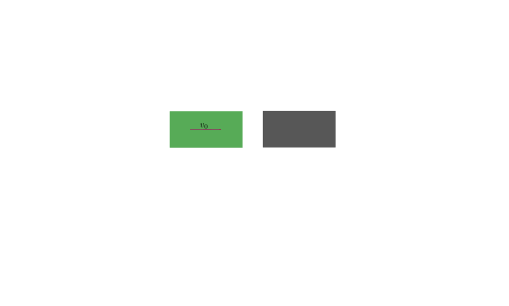
\includegraphics[width=0.8\textwidth]{images/csph/images/yan_2021_linear_interface/schematic}
  \caption{
    Collision between two rectangular elastic solids, where, the left solid is allowed
    to move towards the right solid with a constant velocity $v_0$, while the right
    solid is at rest.}
\label{fig:results-yan-linear-interface-schematic}
\end{figure}
\begin{table}[!ht]
  \centering
  \begin{tabular}[!ht]{ll}
    \toprule
    Quantity & Values\\
    \midrule
    $h/\Delta x$, Smoothing length factor & 1\\
    $\alpha$, artificial viscosity & $1$ \\
    $\beta$, artificial viscosity & $0$ \\
    $k_r$, Normal stiffness coefficient & $10^{11}$ \\
    $k_f$, Tangential stiffness coefficient & $10^{9}$ \\
    \bottomrule
  \end{tabular}
  \caption{Numerical parameters used for the impact of linear interface problem.}%
  \label{tab:linear-interface-numerical-params}
\end{table}

\Cref{fig:results-yan-linear-velocity-vs-time} shows the velocity of the
center of mass of both the bodies using current scheme along with the
formulation of \cite{gray2001sph} and with FEM results provided by
\cite{yan2021simulation}. From the
\cref{fig:results-yan-linear-velocity-vs-time} we can see that rebound
velocities match well with the FEM results provided, as well as the
interaction between the bodies start when their physical boundaries have come
into contact, in contrast to SPH, where the bodies interact when the other
body is in its smoothing length influence. The rebound velocity of the current
scheme is matches well with FEM result. Since the body is elastic,
after the collision, both the bodies move with the base oscillation amplitude
% \todoin{Try to explain oscillation amplitude}
which is the reason why the left body does not achieve a zero velocity.
The current scheme results are better than the CTVF model.
\begin{figure}[!htpb]
  \centering
  \includegraphics[width=0.6\textwidth]{figures/csph/figures/yan_2021_linear_interface/velocity_vs_time}
  \caption{Time history of the x component of the center of mass's velocity of
    the left and the right rectangular bodies, and compared with the numerical
    results produced using FEM, SPH.}
\label{fig:results-yan-linear-velocity-vs-time}
\end{figure}


\FloatBarrier%
\subsection{Colliding rubber rings}
\label{sec:results-rings}
This test applies the current solver in modeling large deformation solids
under collision. We consider the collision between two elastic rubber rings.
This benchmark is simulated by various works in SPH literature, such as in
\cite{gray2001sph,adepu2021corrected,zhang2017generalized}.

\begin{figure}[!htpb]
  \centering
  \includegraphics[width=0.7\textwidth]{images/csph/images/yan_2021_colliding_rubber_rings/schematic}
  \caption{Schematic sketch of the initial setup of colliding rubber rings.}
\label{fig:colliding_rings}
\end{figure}
The initial positioning, as well as the dimensions of the rings, are shown in
\cref{fig:colliding_rings}. Both rings are made of the same material, whose
material properties are listed in \cref{tab:colliding-rings-material-params},
and the numerical parameters in \cref{tab:colliding-rings-numerical-params},
respectively. The initial relative velocity at which the rings collide is
$v_0 = 0.12 c_0$ m\,s\textsuperscript{-1}.

\begin{table}[!ht]
  \centering
  \begin{tabular}[!ht]{ll}
    \toprule
    Quantity & Values\\
    \midrule
    $E$, Young's modulus & $10$ MPa \\
    $\nu$, Poisson's ratio & $0.47$ \\
    $\rho$, density & $1200$ kg\,m\textsuperscript{-3} \\
    $\mu$, friction coefficient & $0.0$ \\
    Time of simulation & $0.016$ s \\
    Resolution, $\delta x$ & $0.001$ m\\
    Smoothing length factor, $h/\Delta x$ & 1.3\\
    gravity $[g_x, g_y, g_z]$ & $[0.0, 0.0, 0.0]$\\
    \bottomrule
  \end{tabular}
  \caption{Material parameters used for modeling the impact of elastic rubber rings.}%
  \label{tab:colliding-rings-material-params}
\end{table}

\begin{table}[!ht]
  \centering
  \begin{tabular}[!ht]{ll}
    \toprule
    Quantity & Values\\
    \midrule
    $\alpha$, artificial viscosity & $1$ \\
    $\beta$, artificial viscosity & $0$ \\
    $k_r$, Normal stiffness coefficient & $10^{7}$ \\
    $k_f$, Tangential stiffness coefficient & $10^{5}$ \\
    \bottomrule
  \end{tabular}
  \caption{Numerical parameters used for modeling the impact of elastic rubber rings.}%
  \label{tab:colliding-rings-numerical-params}
\end{table}

The evolution of the rings is shown in \cref{fig:rings:new-ipst-nu-0-47}, we
can see from the figure that the current model has reproduced a stable and
smooth stress field. The rings are stress free before the collision, as shown
in \cref{fig:rings:ipst-nu-0.47-1}. Throughout the simulation phase, while the
rings are colliding, the kinetic energy of the rings is transferred into
elastic and vice versa. At the maximum deformation, the elastic energy stored
in the rings is maximum. After that, both the rings bounce off and start to
separate. Further, we can see the rings being under tension as well as
compression, while it is deforming in \cref{fig:rings:ipst-nu-0.47-3}. The
results are consistent with other numerical methods proposed by
\cite{gray2001sph} and \cite{zhang2017generalized}.
\begin{figure}[!htpb]
  \centering
  \begin{subfigure}{0.48\textwidth}
    \centering
    \includegraphics[width=1.0\textwidth]{figures/csph/figures/yan_2021_colliding_rubber_rings/poisson_ratio_0_47/time0}
    \subcaption{t = $0$ ms}\label{fig:rings:ipst-nu-0.47-1}
  \end{subfigure}
  %
  \begin{subfigure}{0.48\textwidth}
    \centering
    \includegraphics[width=1.0\textwidth]{figures/csph/figures/yan_2021_colliding_rubber_rings/poisson_ratio_0_47/time1}
    \subcaption{t = $1.38$ ms}\label{fig:rings:ipst-nu-0.47-2}
  \end{subfigure}

  \begin{subfigure}{0.48\textwidth}
    \centering
    \includegraphics[width=1.0\textwidth]{figures/csph/figures/yan_2021_colliding_rubber_rings/poisson_ratio_0_47/time2}
    \subcaption{t = $5.17$ ms}\label{fig:rings:ipst-nu-0.47-3}
  \end{subfigure}
%
  \begin{subfigure}{0.48\textwidth}
    \centering
    \includegraphics[width=1.0\textwidth]{figures/csph/figures/yan_2021_colliding_rubber_rings/poisson_ratio_0_47/time3}
    \subcaption{t = $7.38$ ms}\label{fig:rings:ipst-nu-0.47-4}
  \end{subfigure}

  \begin{subfigure}{0.48\textwidth}
    \centering
    \includegraphics[width=1.0\textwidth]{figures/csph/figures/yan_2021_colliding_rubber_rings/poisson_ratio_0_47/time4}
    \subcaption{t = $11.462$ ms}\label{fig:rings:ipst-nu-0.47-3}
  \end{subfigure}
%
  \begin{subfigure}{0.48\textwidth}
    \centering
    \includegraphics[width=1.0\textwidth]{figures/csph/figures/yan_2021_colliding_rubber_rings/poisson_ratio_0_47/time5}
    \subcaption{t = $15.4$ ms}\label{fig:rings:ipst-nu-0.47-4}
  \end{subfigure}
  \caption{Snapshots of particle positions with color indicating the stress
    field ($\sigma_{xx}$) solved by the current solver.}
\label{fig:rings:new-ipst-nu-0-47}
\end{figure}
%

% ====================================================================================
% ====================================================================================
\FloatBarrier%
\subsection{Near miss of two solids}
\label{sec:results-two-solids-passing-by}
In this section, we study the collision behavior of two solids moving toward
each other, initially placed such that they are not touching. The schematic is
shown in \cref{fig:results-solid-passing-by-schematic}. We show that the current
model is able to eliminate the unphysical interaction that arises due to the
conventional SPH, which is due to the physical influence of the particles at the
boundary. We expect no change in the velocity of the elastic solids as they pass
by. We show that with the current model no interaction exists when the elastic
solids are physically not touching, and no variation in their path is found. As
a qualitative validation the particle plots is shown and for quantitative
validation, variation of the velocity of the center of mass of the elastic body
with time is considered.

\begin{figure}[!htpb]
  \centering
  \includegraphics[width=0.7\textwidth]{images/csph/images/dinesh_2022_elastic_solids_passing_by/schematic}
  \caption{Schematic of the two elastic solids which are placed close to each
    other and allowed to move at a constant velocity $v_0$ with opposite signs.}
\label{fig:results-solid-passing-by-schematic}
\end{figure}
The dimensions of the elastic bodies under consideration are as follows, the
length and height are $0.2$ m and $0.1$ m, respectively. Both bodies are made
of density $1200$ kg\,m\textsuperscript{-3}, Young��s modulus of $10$ MPa and
Poisson��s ratio of $0.4$. The left body is allowed to
move to the right in the x-direction with a velocity of $v_0=20$
m\,s\textsuperscript{-1}, and the right body with $v_0=-20$
m\,s\textsuperscript{-1}. A particle spacing of dx $=0.0025$ m is used, which
results in 3321 particles per single body. We have turned off the particle
shifting in the current test case as no deformation of the bodies is expected.

\begin{figure}[!htpb]
  \centering
  \begin{subfigure}{0.48\textwidth}
    \centering
    \includegraphics[width=1.0\textwidth]{figures/csph/figures/dinesh_2022_elastic_solids_passing_by/CTVF/time0}
    \subcaption{t = $0$ ms}\label{fig:passing-0}
  \end{subfigure}
  %
  \begin{subfigure}{0.48\textwidth}
    \centering
    \includegraphics[width=1.0\textwidth]{figures/csph/figures/dinesh_2022_elastic_solids_passing_by/CTVF/time1}
    \subcaption{t = $1.4$ ms}\label{fig:passing-1}
  \end{subfigure}

  \begin{subfigure}{0.48\textwidth}
    \centering
    \includegraphics[width=1.0\textwidth]{figures/csph/figures/dinesh_2022_elastic_solids_passing_by/CTVF/time2}
    \subcaption{t = $10$ ms}\label{fig:passing-2}
  \end{subfigure}
  %
  \begin{subfigure}{0.48\textwidth}
    \centering
    \includegraphics[width=1.0\textwidth]{figures/csph/figures/dinesh_2022_elastic_solids_passing_by/CTVF/time3}
    \subcaption{t = $12$ ms}\label{fig:passing-3}
  \end{subfigure}
  \caption{Snapshots of the bodies passing close by when simulated with CTVF.}
  \label{fig:dinesh-2022-passing-ctvf}
\end{figure}
%

\begin{figure}[!htpb]
  \centering
  \begin{subfigure}{0.48\textwidth}
    \centering
    \includegraphics[width=1.0\textwidth]{figures/csph/figures/dinesh_2022_elastic_solids_passing_by/Mohseni_Vyas/time0}
    \subcaption{t = $0$ ms}\label{fig:passing-0}
  \end{subfigure}
  %
  \begin{subfigure}{0.48\textwidth}
    \centering
    \includegraphics[width=1.0\textwidth]{figures/csph/figures/dinesh_2022_elastic_solids_passing_by/Mohseni_Vyas/time1}
    \subcaption{t = $1.4$ ms}\label{fig:passing-1}
  \end{subfigure}

  \begin{subfigure}{0.48\textwidth}
    \centering
    \includegraphics[width=1.0\textwidth]{figures/csph/figures/dinesh_2022_elastic_solids_passing_by/Mohseni_Vyas/time2}
    \subcaption{t = $10$ ms}\label{fig:passing-2}
  \end{subfigure}
  %
  \begin{subfigure}{0.48\textwidth}
    \centering
    \includegraphics[width=1.0\textwidth]{figures/csph/figures/dinesh_2022_elastic_solids_passing_by/Mohseni_Vyas/time3}
    \subcaption{t = $12$ ms}\label{fig:passing-3}
  \end{subfigure}
  \caption{Snapshots of the bodies passing close by when simulated with current solver.}
\label{fig:dinesh-2022-passing-collision}
\end{figure}
%
\Cref{fig:dinesh-2022-passing-ctvf} shows the snapshots of bodies at multiple
time instants simulated using the formulation of \cite{adepu2021corrected}.
From \Cref{fig:dinesh-2022-passing-ctvf} we can see that the bodies interact
with each other though they are not touching physically, this is because in
SPH the particles at the boundaries have an influence radius exceeding its
material boundary. Because of the interaction, shear stresses develop, which
results in strain in the body as well as it deviates from its path.
\Cref{fig:dinesh-2022-passing-collision} shows the snapshots of bodies when
simulated with the current contact force model with the current SPH
formulation. From \cref{fig:dinesh-2022-passing-collision}, we can clearly see
that the bodies don't interact and pass freely without any deformations or
path divergence.
\begin{figure}[!htpb]
  \centering
  \includegraphics[width=0.48\textwidth]{figures/csph/figures/dinesh_2022_elastic_solids_passing_by/velocity_vs_time_x}
  \includegraphics[width=0.48\textwidth]{figures/csph/figures/dinesh_2022_elastic_solids_passing_by/velocity_vs_time_y}
  \caption{Time variation of the x-component and y-component of the velocity
    of the center of mass of the freely moving rectangular solids when
    simulated using the CTVF and the current solver.}
\label{fig:results-dinesh-passing-velocity-x-y-vs-time}
\end{figure}
% \begin{figure}[!htpb]
%   \centering
%   \caption{Time variation of the y-component of center of mass velocity of the
%     freely moving left and right rectangular solids when simulated using the
%     CTVF and the current solver.}
% \label{fig:results-dinesh-passing-velocity-y-vs-time}
% \end{figure}
\Cref{fig:results-dinesh-passing-velocity-x-y-vs-time} shows a quantitative
validation by considering the time history of the velocity of the center of
mass in the x and y-direction. From
\cref{fig:results-dinesh-passing-velocity-x-y-vs-time} we can see that the
velocity of the left body, as well as the right body, is constant throughout
the time. While a velocity in the y-direction is induced while simulated using
\cite{adepu2021corrected} formulation. Hence the current scheme is successful
in modeling the free moment of elastic solids passing close by each other.

% ====================================================================================
% ====================================================================================
\FloatBarrier%
\subsection{Elastic solid sliding on a slope}
\label{sec:results-elastic-solid-sliding-on-slope}
In the current problem, we test if the current scheme models the friction
between the elastic solids accurately. The free sliding of an elastic solid on
a frictional inclined plane is studied. The initial placement of the elastic
solid is shown in \cref{fig:results-solid-sliding-schematic}.
\begin{figure}[!htpb]
  \centering
  \includegraphics[width=0.4\textwidth]{figures/csph/figures/mohseni_2021_free_sliding_on_a_slope/fric_coeff_0_4/pre_schematic}
  \caption{Schematic of an elastic body sliding on a frictional slope.}
\label{fig:results-solid-sliding-schematic}
\end{figure}

An elastic solid of length $0.1$ m and width $0.1$ m is initially placed at zero
velocity on an inclined plane at an angle of $30$ degrees. The material
properties are as follows: An Young's modulus of $10$ MPa with a Poisson ratio
of $0.3975$ is considered. We have turned the particle homogenization off in the
current problem, as the particle shifting effects are negligible. A stiffness
coefficient $k_r$ of $10^{10}$ in \cref{eq:contact-algorithm-normal} is used.
From the analytical solution, we have the evolution of velocity as follows,
\begin{equation}
  \label{eq:analytical-sliding-body}
  \ten{v}(t) = (\mu \teng{g} \sin (\theta) - \teng{g} \cos (\theta)) t.
\end{equation}

We consider three different frictional coefficients, $\mu=0.2, 0.3, 0.4$ while
modeling the sliding of the elastic solid. Snapshots at four time instants are
depicted in \cref{fig:mohseni-2021-sliding}, corresponding to the frictional
coefficient of $0.3$. From \cref{fig:mohseni-2021-sliding} we can see that the
elastic solid slides without any oscillations.
\Cref{fig:results-solid-sliding-velocity-vs-time} presents the time history of
the velocity of center of mass of the elastic body along with the
corresponding theoretical solution obtained by frictional coefficients of
$\mu=0.2$, $0.3$, and $0.4$. From
\cref{fig:results-solid-sliding-velocity-vs-time}, the reproduced velocity is
in good agreement with the corresponding theoretical solution for all the
time.
\begin{figure}[!htpb]
  \centering
  \begin{subfigure}{0.48\textwidth}
    \centering
    \includegraphics[width=1.0\textwidth]{figures/csph/figures/mohseni_2021_free_sliding_on_a_slope/fric_coeff_0_3/time0}
    \subcaption{t = $0$ sec}\label{fig:passing-0}
  \end{subfigure}
  %
  \begin{subfigure}{0.48\textwidth}
    \centering
    \includegraphics[width=1.0\textwidth]{figures/csph/figures/mohseni_2021_free_sliding_on_a_slope/fric_coeff_0_3/time1}
    \subcaption{t = $0.5$ sec}\label{fig:passing-1}
  \end{subfigure}

  \begin{subfigure}{0.48\textwidth}
    \centering
    \includegraphics[width=1.0\textwidth]{figures/csph/figures/mohseni_2021_free_sliding_on_a_slope/fric_coeff_0_3/time2}
    \subcaption{t = $1.$ sec}\label{fig:passing-2}
  \end{subfigure}
  %
  \begin{subfigure}{0.48\textwidth}
    \centering
    \includegraphics[width=1.0\textwidth]{figures/csph/figures/mohseni_2021_free_sliding_on_a_slope/fric_coeff_0_3/time3}
    \subcaption{t = $2$ sec}\label{fig:passing-3}
  \end{subfigure}
  \caption{Snapshots of the elastic solid sliding on an inclined plane at
    four time steps, where, the friction coefficient between the body and
    the plane is taken as $0.3$.}
\label{fig:mohseni-2021-sliding}
\end{figure}
%

\begin{figure}[!htpb]
  \centering
  \includegraphics[width=0.4\textwidth]{figures/csph/figures/mohseni_2021_free_sliding_on_a_slope/velocity_vs_time}
  \caption{Time histories of the velocity of the elastic solid while sliding on
    an inclined plane for three frictional coefficients, plotted against the
    analytical solution.}
\label{fig:results-solid-sliding-velocity-vs-time}
\end{figure}


% ====================================================================================
% ====================================================================================
\FloatBarrier%
\subsection{Circular elastic body rolling on a plane}
\label{sec:de-cylinder}

In the current section, the motion of a 2D elastic cylinder rolling on a
frictional inclined plane is carried out. The theoretical and computational
model are shown in \cref{fig:circular-rolling}. In addition to the problem
considered in \cref{sec:results-elastic-solid-sliding-on-slope}, the current
problem will be helpful in testing the frictional part of the current
\begin{figure}[!htpb]
  \centering
  \begin{subfigure}{0.40\textwidth}
    \centering
    \includegraphics[width=1.0\textwidth]{images/csph/images/de_2021_cylinder_rolling_on_an_inclined_plane/schematic_1}
    \subcaption{}\label{fig:circular-rolling-theory}
  \end{subfigure}
  \begin{subfigure}{0.48\textwidth}
    \centering
    \includegraphics[width=1.0\textwidth]{images/csph/images/de_2021_cylinder_rolling_on_an_inclined_plane/schematic_2}
    \subcaption{}\label{fig:circular-rolling-computational}
  \end{subfigure}
  \caption{The rolling body problem: (a) theoretical description (b) numerical model.}
\label{fig:circular-rolling}
\end{figure}
formulation. A total of two coefficient of friction $\mu$ values are
simulated. One with a slip case ($\mu=0.3$) and with $\mu=0.6$ corresponding
to stick case, where the inclination of the plane is chosen to be
$\theta=\pi/3$. \Cref{tab:circular-cylinder-rolling} shows the material
properties along with numerical parameters utilized in the current scheme. The
analytical solution of the movement of the center of the circular body for
different frictional coefficients is given as
\begin{align}
  \label{eq:analytical-x-cm-rolling-cylinder}
  x_{cm}(t) =
  \begin{cases}
  x_0 + \frac{1}{2} \, g \, t^2 \, (\sin(\theta) - \mu \cos(\theta)) & \tan{\theta} > 3.5\mu,\\
  x_0 + \frac{1}{3} \, g \, t^2 \, \sin(\theta) & \tan{\theta} \leq 3.5\mu.
\end{cases}
\end{align}
Here, $g=9.81$ is the magnitude of acceleration due to gravity.

\begin{table}[!ht]
  \centering
  \begin{tabular}[!ht]{ll}
    \toprule
    Quantity & Values\\
    \midrule
    $E$, Young's modulus & $10$ MPa \\
    $\nu$, Poisson's ratio & $0.3975$ \\
    $\rho$, density & $1200$ kg\,m\textsuperscript{-3} \\
    $\mu$, friction coefficient & $0.3$ \& $0.6$ \\
    Time of simulation & $0.6$ s \\
    Resolution, $\delta x$ & $0.0025$ m\\
    Smoothing length factor, $h/\Delta x$ & 1.3\\
    gravity $[g_x, g_y, g_z]$ & $[g\,\sin(\theta), g\,\cos(\theta), 0.0]$\\
    $\alpha$, artificial viscosity & $1$ \\
    $\beta$, artificial viscosity & $0$ \\
    $k_r$, Normal stiffness coefficient & $10^{7}$ \\
    $k_f$, Tangential stiffness coefficient & $10^{5}$ \\
    \bottomrule
  \end{tabular}
  \caption{Numerical parameters and material properties for the rolling circular
    cylinder.}%
  \label{tab:circular-cylinder-rolling}
\end{table}

%
%
\begin{figure}[!htpb]
  \centering
  \begin{subfigure}{0.48\textwidth}
    \centering
    \includegraphics[width=1.0\textwidth]{figures/csph/figures/de_2021_cylinder_rolling_on_an_inclined_plane/fric_coeff_0_3/time0}
    \subcaption{}
  \end{subfigure}
  \begin{subfigure}{0.48\textwidth}
    \centering
    \includegraphics[width=1.0\textwidth]{figures/csph/figures/de_2021_cylinder_rolling_on_an_inclined_plane/fric_coeff_0_3/time1}
    \subcaption{}
  \end{subfigure}
  \caption{Snapshot of a rolling cylinder with the velocity vectors at two
    time steps for a friction coefficient of $0.3$, corresponding to a slip
    case.}
\label{fig:de-2021-rolling-mu-0-3}
\end{figure}
%
\begin{figure}[!htpb]
  \centering
  \begin{subfigure}{0.48\textwidth}
    \centering
    \includegraphics[width=1.0\textwidth]{figures/csph/figures/de_2021_cylinder_rolling_on_an_inclined_plane/fric_coeff_0_6/time0}
    \subcaption{}
  \end{subfigure}
  \begin{subfigure}{0.48\textwidth}
    \centering
    \includegraphics[width=1.0\textwidth]{figures/csph/figures/de_2021_cylinder_rolling_on_an_inclined_plane/fric_coeff_0_6/time1}
    \subcaption{}
  \end{subfigure}
  \caption{Snapshot of a rolling cylinder with the velocity vectors at two
    time steps for a friction coefficient of $0.6$, corresponding to a stick
    case.}
\label{fig:de-2021-rolling-mu-0-6}
\end{figure}
%
\begin{figure}[!htpb]
  \centering
  \includegraphics[width=0.6\textwidth]{figures/csph/figures/de_2021_cylinder_rolling_on_an_inclined_plane/fric_coeff_0_3/xcom_vs_time}
  \caption{Time variation of the x-component of the center of mass of the
    circular cylinder for a friction coefficient of $0.3$.}
\label{fig:results-cylinder-rolling-fric-coeff-0-3-xcom-vs-time}
\end{figure}
%
\begin{figure}[!htpb]
  \centering
  \includegraphics[width=0.6\textwidth]{figures/csph/figures/de_2021_cylinder_rolling_on_an_inclined_plane/fric_coeff_0_6/xcom_vs_time}
  \caption{Time variation of the x-component of the center of mass of the
    circular cylinder for a friction coefficient of $0.6$.}
\label{fig:results-cylinder-rolling-fric-coeff-0-6-xcom-vs-time}
\end{figure}
\Cref{fig:de-2021-rolling-mu-0-3} and \Cref{fig:de-2021-rolling-mu-0-6} shows
the snapshots of the cylinder at two different time instants along with the
scaled velocity vectors for friction coefficients $\mu=0.3$ and $0.6$
respectively. Finally,
\cref{fig:results-cylinder-rolling-fric-coeff-0-3-xcom-vs-time} and
\cref{fig:results-cylinder-rolling-fric-coeff-0-6-xcom-vs-time} depicts the x
position of the center of mass of the cylinder along with time for a slip and
stick case. From these figures, we can see that the current scheme agrees well
with the analytical solution.

% ====================================================================================
% ====================================================================================
\FloatBarrier%
\subsection{A rigid sphere hitting a wall at different impact angles}
\label{sec:r-vyas}
\begin{figure}[!htpb]
  \centering
  \includegraphics[width=0.6\textwidth]{images/csph/images/vyas_2021_rebound_kinematics_3d/schematic}
  \caption{3d rigid body rebound schematic}
\label{fig:results-vyas-3d-rebound-schematic}
\end{figure}
In the current example, we simulate the impact of a 3D sphere on a wall at
different incident angles, where the experimental evaluation is done by
\cite{thornton2011investigation}. The model description is shown in
\cref{fig:results-vyas-3d-rebound-schematic}. The sphere is assumed to be
rigid and the material properties as well as the numerical parameters used are
displayed in \cref{tab:sphere-wall-impact}. The sphere is impacted on the wall
by varying the incident angles ($\theta_i$) keeping the magnitude of the
velocity constant, $5$ m\,s\textsuperscript{-1}.
\begin{table}[!ht]
  \centering
  \begin{tabular}[!ht]{ll}
    \toprule
    Quantity & Values\\
    \midrule
    $E$, Young's modulus & $70$ GPa \\
    $\nu$, Poisson's ratio & $0.3$ \\
    $\rho$, density & $2650$ kg\,m\textsuperscript{-3} \\
    $\mu$, friction coefficient & $0.1$ \\
    Time of simulation & $0.25$ ms \\
    Resolution, $\delta x$ & $0.00153$ m\\
    Smoothing length factor, $h/\Delta x$ & 1.0\\
    gravity $[g_x, g_y, g_z]$ & $[0.0, -9.81, 0.0]$\\
    $k_r$, Normal stiffness coefficient & $10^{7}$ \\
    $k_f$, Tangential stiffness coefficient & $10^{5}$ \\
    \bottomrule
  \end{tabular}
  \caption{Numerical parameters and material properties for sphere impacting a wall.}%
  \label{tab:sphere-wall-impact}
\end{table}

\begin{figure}[!htpb]
  \centering
  \includegraphics[width=0.6\textwidth]{figures/csph/figures/vyas_2021_rebound_kinematics_3d/theta_vs_omega}
  \caption{The plot of the variation of $\omega^*_r$ with $\theta^*_i$ of the
    impacting sphere simulated with the current numerical scheme, compared
    with the experimental result by \cite{thornton2011investigation}.}
\label{fig:results-sphere-impact-theta-vs-omega}
\end{figure}
\Cref{fig:results-sphere-impact-theta-vs-omega} depicts the variation of the
non-dimensional angular velocity $\omega^*_r$ against the non-dimensional
incident angle $\theta^{*}_i$, where $\theta^{*}$ and $\omega^*_r$ are defined as
\begin{equation}
  \label{eq:non-dim-theta}
  \theta^{*}_i = \frac{2 \tan(\theta_i)}{(1 + e_n) \mu},
\end{equation}
\begin{equation}
  \label{eq:non-dim-omega}
  \omega^{*}_r = \frac{2\,R\,\omega_r}{(1 + e_n) \, \mu \, V_{ni}},
\end{equation}
respectively. Here, $\omega_r$ corresponds to the z-component of the angular
velocity vector. The simulated results are compared to the experimental
results by \cite{thornton2011investigation}. From the
\cref{fig:results-sphere-impact-theta-vs-omega}, we can see that the current
solver is able to replicate the original behavior to an acceptable
degree. We observe that the variation of the $\omega^{*}_r$ with
$\theta^{*}_i$ to be linear with the current solver whereas the experimental
result to be a nonlinear, this may be due to the usage of the linear force model
in the current scheme.


\FloatBarrier%
\subsection{Stress wave propagation in granular media}
\label{sec:results-stress-wave-propagation-with-friction}
\begin{figure}[!htpb]
  \centering
  \includegraphics[width=1.0\textwidth]{images/csph/images/de_2021_stress_wave_in_granular_material_part_2/schematic}
  \caption{Schematic of the initial placement of the frictional granular media including the impactor and walls}
\label{fig:results-stress-wave-propagation-part-II}
\end{figure}
So far, we have modeled the collision between two bodies, in the current
section, we study the collision among multiple bodies. The elastic wave
propagation in a granular media is carried out, and whose experimental study was
executed by \cite{guilkey2001improved}. To our knowledge this problem has not
yet been performed in SPH literature yet. We consider five identical disks
placed at an angle of $45$ degrees, allowed to be impacted by a moving wall from
right with a velocity $5.6$ m\,s\textsuperscript{-1} in horizontal direction as
depicted in \cref{fig:results-stress-wave-propagation-part-II}. Each granular
disk has a radius of $50$ mm, which are initially placed such that they are just
touching. A particle spacing of $1.25$ mm is used, which results in $7830$
particles per disk. The rigid box are modelled as rigid surfaces. The material
parameters of the disc as well as the numerical parameters used in the numerical
simulation are listed in \cref{tab:de-stress-part-2-params}.
\begin{table}[!ht]
  \centering
  \begin{tabular}[!ht]{ll}
    \toprule
    Quantity & Values\\
    \midrule
    $K$, Bulk modulus & $102$ GPa \\
    $G$, Shear modulus & $72$ GPa \\
    $\rho$, density & $1900$ kg\,m\textsuperscript{-3} \\
    gravity $[g_x, g_y, g_z]$ & $[0.0, 0.0, 0.0]$\\
    $k_r$, Normal stiffness coefficient & $1.75 \times 10^{11}$ \\
    $k_f$, Tangential stiffness coefficient & $5 \times 10^{10}$ \\
    $\mu$, Friction coefficient & 0.5 \\
    \bottomrule
  \end{tabular}
  \caption{Material and numerical parameters used for the stress wave propagation problem.}%
  \label{tab:de-stress-part-2-params}
\end{table}
\Cref{fig:de-stress-wave-compare} shows the particle plots of the granular
discs with the stress fringes from the experiment \citep{guilkey2001improved},
and the simulation carried in the present study, and from the numerical study
of \cite{de2021modelling}, where the simulation is carried out using a total
Lagrangian material point method (TLMPM). The snapshots of the current work
are taken at time $0.2$ ms, while the results of experimental and TLMPM result
correspond to the time at $0.12$ ms. This is due to the initial placement of
the discs in the current work and the stress fringes being sensitive to
initial placement. Here, the stress fringes in the experimental work are
evaluated using photo-elasticity. While, in the numerical work, the fringes
are generated by plotting $\sigma_f$, computed as:
\begin{equation}
  \label{eq:stress-fringe-formula}
  \sigma_f = 1 - \sin^2(f (\sigma_1 - \sigma_3)),
\end{equation}
where $f$ is a optical parameter which controls the fringe density, taken as $\pi/0.07$
G\,Pa\textsuperscript{-1}. The difference in the in-plane principal stress is computed using,
\begin{equation}
  \label{eq:principal-stress-difference}
  \sigma_1 - \sigma_3 = 2R = \sqrt{4 \tau_{xy}^2 + (\sigma_x - \sigma_y)^2}
\end{equation}
\begin{figure}[!htpb]
  \centering
  \begin{subfigure}{1.0\textwidth}
    \centering
    \includegraphics[width=0.7\textwidth]{images/csph/images/de_2021_stress_wave_in_granular_material_part_2/bardenhagen_2001}
    \subcaption{}\label{fig:de-stress-wave-bardenhagen}
  \end{subfigure}

  \begin{subfigure}{1.0\textwidth}
    \centering
    \includegraphics[width=0.7\textwidth]{images/csph/images/de_2021_stress_wave_in_granular_material_part_2/tlmpm_2021}
    \subcaption{}\label{}
  \end{subfigure}

  \begin{subfigure}{1.0\textwidth}
    \centering
    \includegraphics[width=0.8\textwidth]{figures/csph/figures/de_2021_stress_wave_in_granular_material_part_2/case_mohseni/time0}
    \subcaption{}\label{fig:de-stress-wave-current}
  \end{subfigure}
  \caption{Stress fringes of the granular discs from (a) experiment
    \citep{guilkey2001improved}, (b) TLMPM \citep{de2021modelling} (c) Current work}
\label{fig:de-stress-wave-compare}
\end{figure}
From the qualitative comparison of the stress fringes in the granular discs of
the current scheme with the experimental as well as the numerical result of
TLMPM, the current scheme fringes are smooth and are similar to the
experimental result.

\FloatBarrier%
\subsection{Primary secondary analysis}
\label{sec:results-primary-secondary-analysis}

In the current section we have studied the dependence of the behaviour of the
current contact force model on the variation of different bodies being primary.
We have considered the following examples:
\begin{itemize}
\item Collision between symmetric bodies
\item Circular cylinder rolling down an inclined plane
\item Square solid sliding down an inclined plane
\item Impact of a 3D sphere against a target wall.
\end{itemize}
\Cref{fig:primary-secondary-four-examples} depicts the variation of velocity
or position of the elastic bodies involved in above cases. From
\cref{fig:primary-secondary-four-examples} we can see that the velocities of
the elastic solids in a symmetric collision are invariant to the primary body
chosen. While, considering the wall as primary in rolling cylinder, and
sliding solid case, the error is more compared to the body being taken as
primary. In the case of granular particle impacting a wall, the angular
velocity of the granular particle deviates from the experimental result when
the wall being the primary body. With these results, we conclude that body
with more curvature is more suitable to take as primary.
\begin{figure}[!htpb]
  \centering
  \begin{subfigure}{0.48\textwidth}
    \centering
    \includegraphics[width=1.\textwidth]{figures/csph/figures/yan_2021_linear_interface_primary_vs_secondary/mohseni_vyas_primary_left_velocity_vs_time}
    \caption{Collision between a flat interface solids.}\label{fig:results-yan-linear-primary-vs-secondary}
  \end{subfigure}
  \begin{subfigure}{0.48\textwidth}
    \centering
    \includegraphics[width=1.\textwidth]{figures/csph/figures/mohseni_2021_free_sliding_on_a_slope_primary_vs_secondary/mohseni_primary_body_velocity_vs_time}
    \caption{An elastic body sliding down an inclined plane}\label{fig:mps}
  \end{subfigure}

  \begin{subfigure}{0.48\textwidth}
    \centering
    \includegraphics[width=1.\textwidth]{figures/csph/figures/de_2021_cylinder_rolling_on_an_inclined_plane_primary_vs_secondary/mohseni_primary_body_xcom_vs_time}
    \caption{A circular cylinder rolling on an inclined plane}\label{fig:rps}
  \end{subfigure}
  \begin{subfigure}{0.48\textwidth}
    \centering
    \includegraphics[width=1.\textwidth]{figures/csph/figures/vyas_2021_rebound_kinematics_3d_compare_flipped/theta_vs_omega}
    \caption{Variation of the angular velocity with respect to the incident
      theta.}\label{fig:vps}
  \end{subfigure}
  \caption{}
\label{fig:primary-secondary-four-examples}
\end{figure}



\FloatBarrier%
\section{Discussions and Summary}

In this chapter we have demonstrated a simple approach to effectively handle the
collision between elastic solids modeled using an updated Lagrangian SPH
model. A contact force model is used to handle the collision between bodies. A
surface aware spring based contact force is used to handle the collision
between bodies. This effectively allows us to model collision and friction
accurately. In addition this eliminates any spurious forces that are commonly
seen with SPH when two bodies are nearby but not in actual contact. The
contact force model utilized in the current work is sensitive towards the
primary and the secondary body chosen. A careful analysis is carried out to
understand which body is to be considered as primary among the colliding
solids, and it is found that choosing the body with the highest curvature as
the primary body gives the best results. Further, we have made our
implementation open-source.

It has been demonstrated that the current model is able to predict the post
collision behaviour of the colliding bodies by simulating collision between
flat, and curved interfaces in two and three dimensions. A sliding elastic
body is simulated to test the frictional part of the contact model. Finally,
the full scale model is applied to model the stress propagation in granular
discs for the first time in SPH. The results compare well with those of FEM as
well as analytical studies.

% A non-linear contact force model can be implemented in the future work. The
% current work can be easily extended to the modeling of collision between
% elastic and elastic-plastic bodies. Also, the collision between the bodies
% undergoing breakage can be easily captured with the current framework.

We have incorporated a contact force model in the current chapter to handle the
collision between arbitrarily shaped elastic solids. This chapter's work in
handling collision is extended to the rigid-elastic and rigid-plastic contacts
in the next few chapters. We have modeled the elastic dynamics, fluid dynamics,
and the collision between the impacting solids with our aim of handling problems
such as abrasive water jet machining. In the next chapter, we will model the
interaction between the fluid and the elastic structure, fluid-structure
interaction, as this is seen when the water from the inlet impacts the target.
We propose an updated Lagrangian solver by coupling the solver developed in
\cref{chap:ctvf} and handling fluid-structure interaction.
